\newpage
\section{Collection of Impliction DAGs}
\label{sec:dags}

All figures have equal entitlements unless specified otherwise.

\begin{figure*}[!htb]
\centering
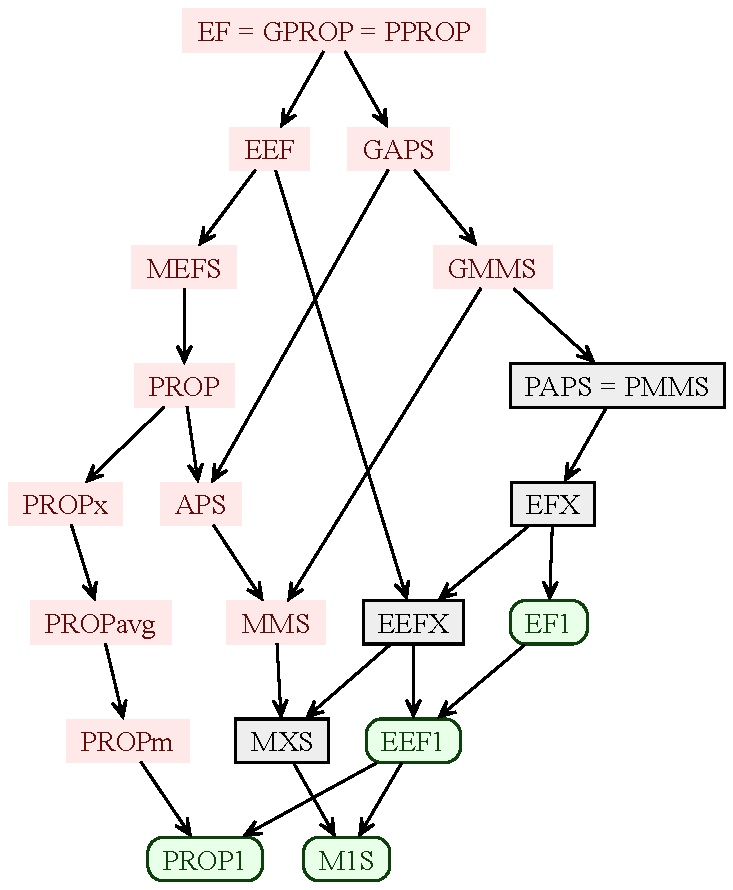
\includegraphics[scale=0.8]{dags/additive-general-0-0-1.pdf}
\caption{Additive valuations, mixed manna.}
\label{fig:additive-general-nny}
\end{figure*}

\begin{figure*}[!htb]
\centering
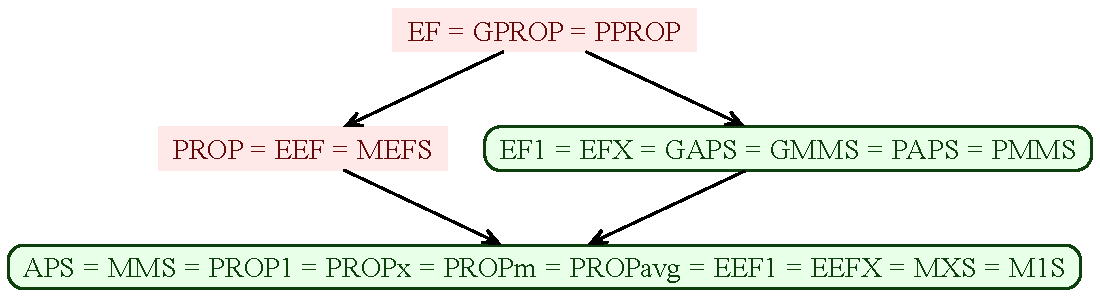
\includegraphics[scale=0.8]{dags/additive-tribool-0-0-1.pdf}
\caption[Additive valuations, triboolean marginals]{%
Additive valuations, marginals in $\{-1, 0, 1\}$.
We get the same DAG when marginals are in $\{0, -1\}$ or $\{0, 1\}$.}
\label{fig:additive-tribool-nny}
\end{figure*}

\begin{figure*}[!htb]
\centering
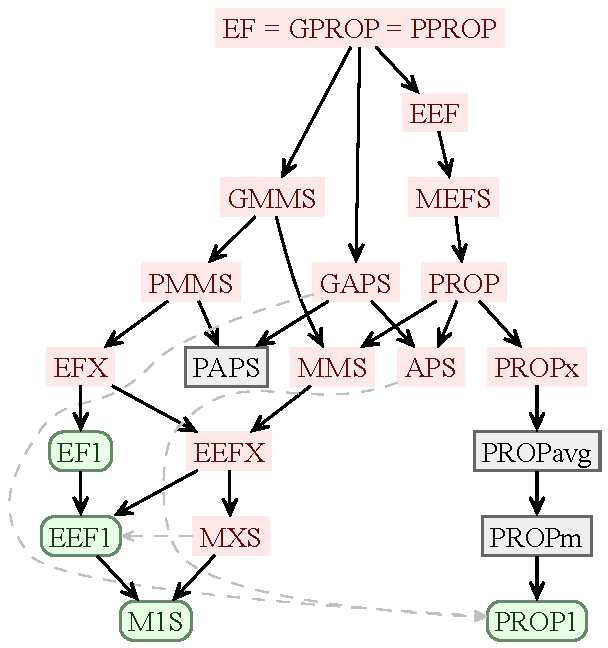
\includegraphics[scale=0.8]{dags/additive-nonneg-0-0-0.pdf}
\caption{Additive valuations, goods, unequal entitlements.}
\label{fig:additive-nonneg-nnn}
\end{figure*}

\begin{figure*}[!htb]
\centering
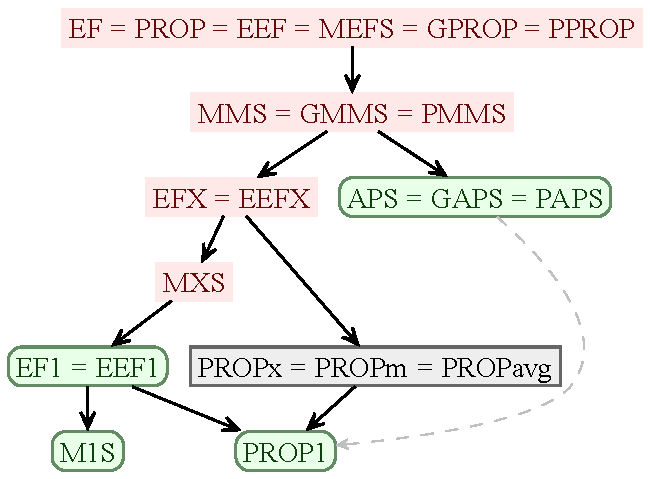
\includegraphics[scale=0.8]{dags/additive-nonneg-0-1-0.pdf}
\caption{Additive valuations, goods, two agents, unequal entitlements.}
\label{fig:additive-nonneg-nyn}
\end{figure*}

\begin{figure*}[!htb]
\centering
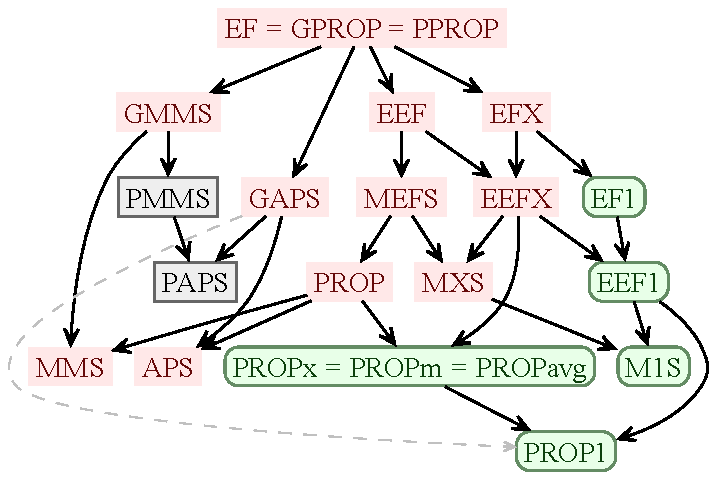
\includegraphics[scale=0.8]{dags/additive-nonpos-0-0-0.pdf}
\caption{Additive valuations, chores, unequal entitlements.}
\label{fig:additive-nonpos-nnn}
\end{figure*}

\begin{figure*}[!htb]
\centering
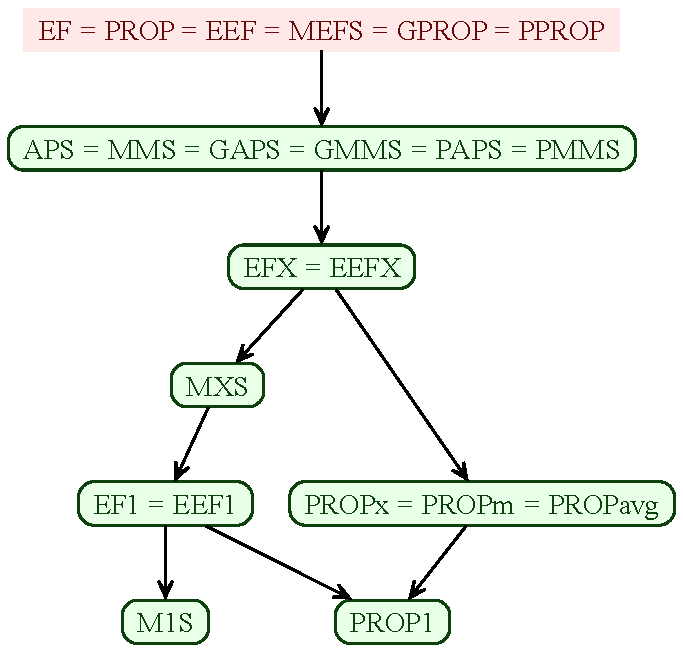
\includegraphics[scale=0.8]{dags/additive-general-0-1-1.pdf}
\caption{Additive valuations, two agents.
We get the same DAG for goods, chores, and mixed manna.}
\label{fig:additive-general-nyy}
\end{figure*}

\begin{figure*}[!htb]
\centering
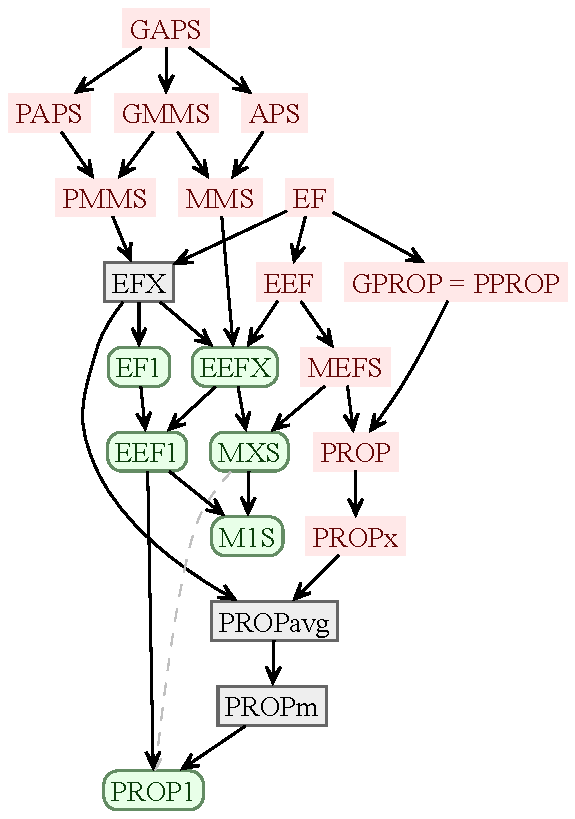
\includegraphics[scale=0.8]{dags/submod-nonneg-0-0-1.pdf}
\caption{Submodular valuations, goods.}
\label{fig:submod-nonneg-nny}
\end{figure*}

\begin{figure*}[!htb]
\centering
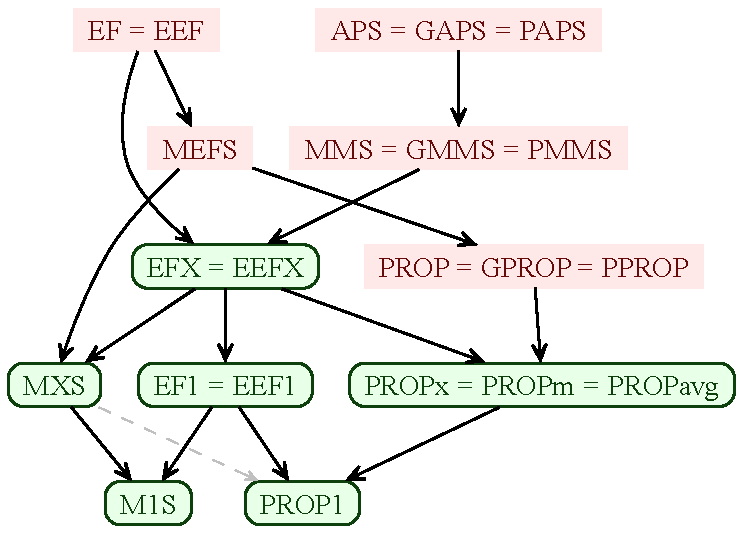
\includegraphics[scale=0.8]{dags/submod-nonneg-0-1-1.pdf}
\caption{Submodular valuations, goods, two agents.}
\label{fig:submod-nonneg-nyy}
\end{figure*}

\begin{figure*}[!htb]
\centering
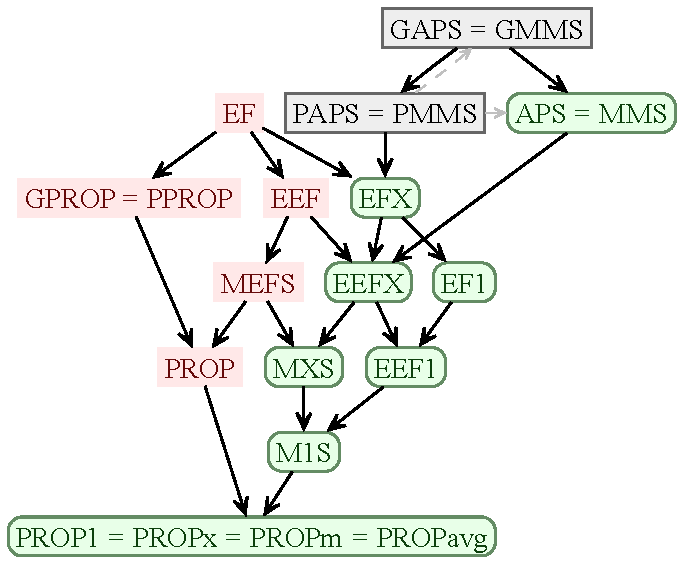
\includegraphics[scale=0.8]{dags/submod-binary-0-0-1.pdf}
\caption{Submodular valuations with binary marginals (a.k.a. matroid rank valuations), goods.}
\label{fig:submod-binary-nny}
\end{figure*}

\begin{figure*}[!htb]
\centering
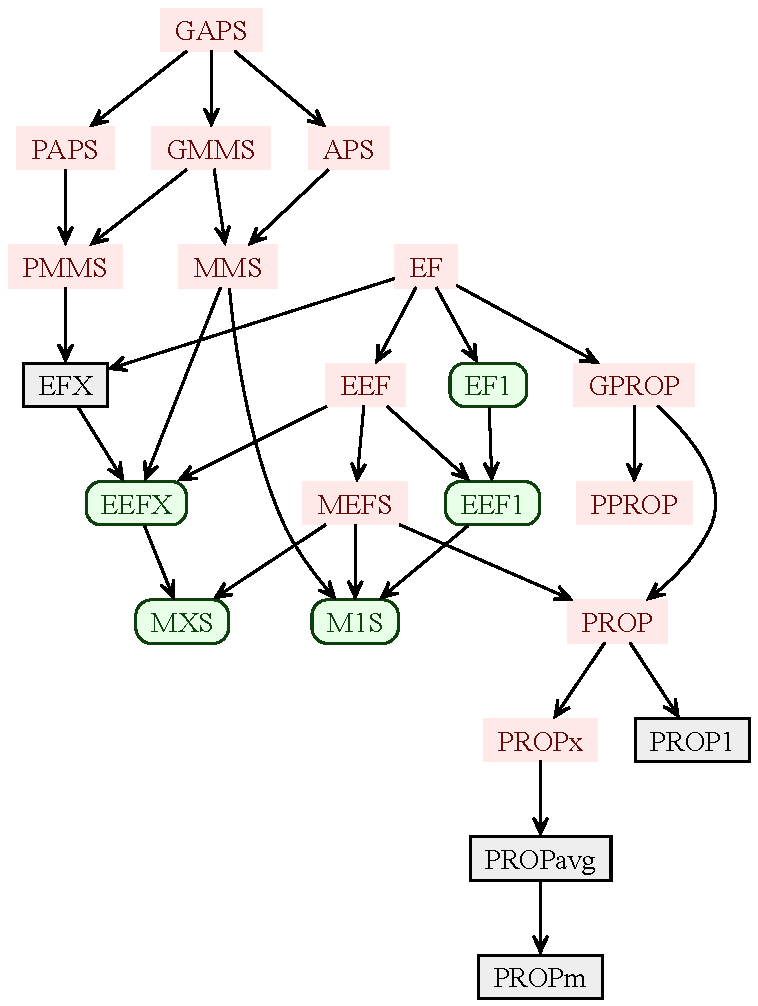
\includegraphics[scale=0.8]{dags/subadd-nonneg-0-0-1.pdf}
\caption{Subadditive valuations, goods.}
\label{fig:subadd-nonneg-nny}
\end{figure*}

\begin{figure*}[!htb]
\centering
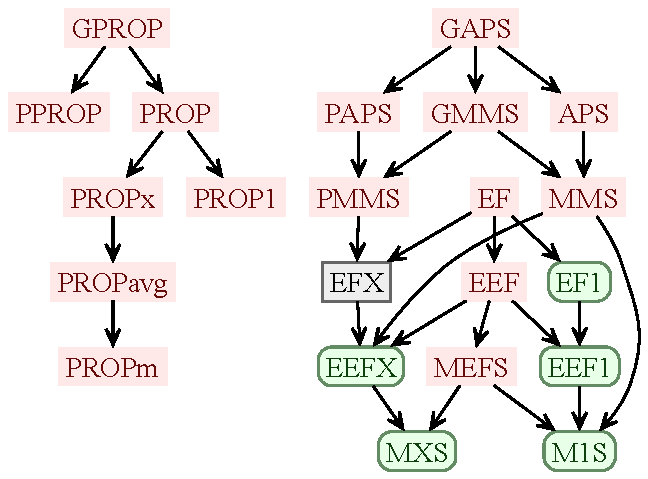
\includegraphics[scale=0.8]{dags/general-nonneg-0-0-1.pdf}
\caption{General (monotonic) valuations, goods.}
\label{fig:general-nonneg-nny}
\end{figure*}

\begin{figure*}[!htb]
\centering
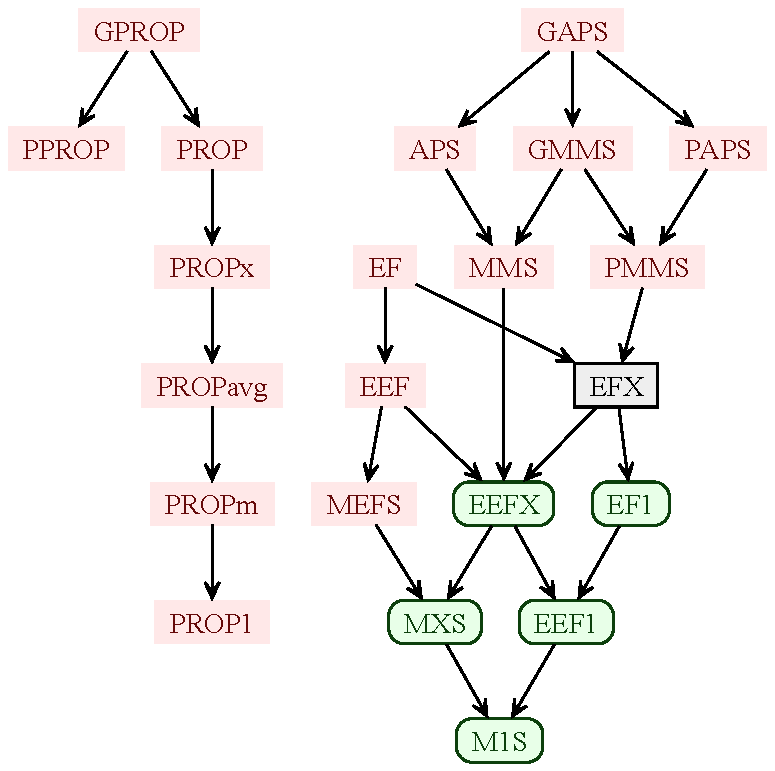
\includegraphics[scale=0.8]{dags/general-positive-0-0-1.pdf}
\caption[General valuations with positive marginals]{%
General valuations with positive marginals.
This setting is almost the same as \cref{fig:general-nonneg-nny},
where marginals are non-negative instead.}
\label{fig:general-positive-nny}
\end{figure*}
